
\section{Explicação do programa}

Aqui irei explicar o funcionamento do programa.
Para tal, primeiro irei apresentar um fluxograma.
Depois será feito uma explicação detalhada.
De qualquer forma, no próprio código tem vários comentários explicando a lógica por tráz do programa.

\subsection{Fluxograma}

\begin{figure}[H]
\centering
%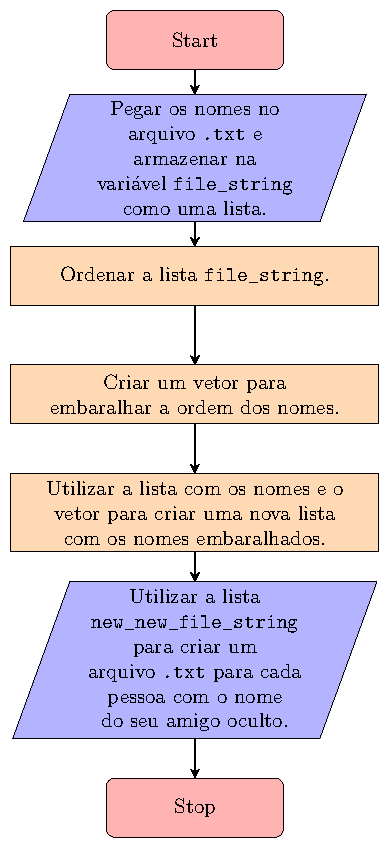
\includegraphics{00_7_imagem_1}
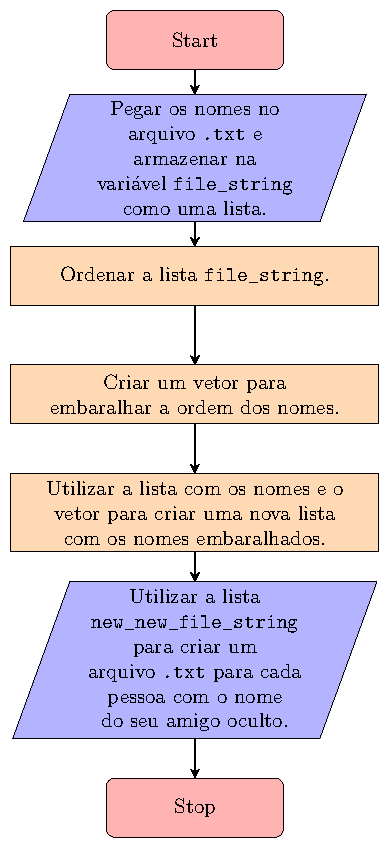
\includegraphics[scale=1.4]{00_7_imagem_1}
%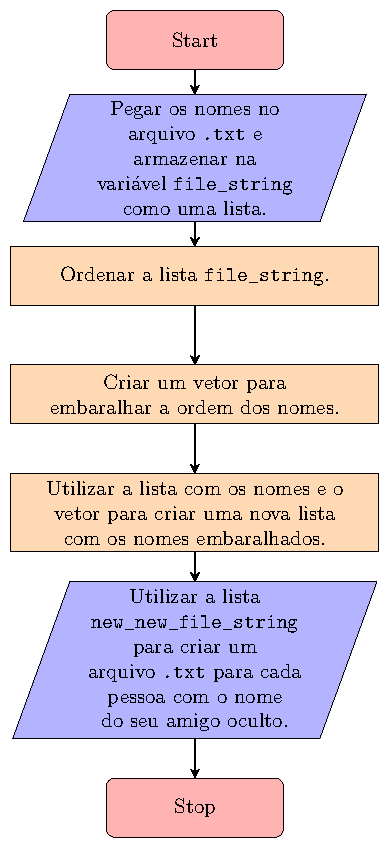
\includegraphics[width=.5\textwidth]{00_7_imagem_1}
\caption{Fluxograma do programa.}
\end{figure}

\newpage

\subsection{Explicação mais detalhada}

Aqui estarei explicando o programa.
Antes, quero dizer que existe mais de uma forma de se fazer as coisas que eu fiz, e que essa é a versão 1.
Além disso, que terá outras versões em que as coisas funcionarão de forma diferente.

No pedaço de código abaixo abrimos o arquivo \texttt{.txt} com os nomes das pessoas e armazenamos cada nome como um elemento de uma lista.
Utilizamos dessa forma porque se tivermos algum problema enquanto o arquivo está aberto ele vai fechar.
Tem outra forma de abrir um arquivo, mas que não fecha automaticamente, e com isso, dessa outra forma, acabamos tendo de lembrar de fechar o arquivo, além disso se tivermos algum problema enquanto o arquivo está aberto ele não vai fechar e podemos ter problemas quanto a isso.

\begin{lstlisting}[
				   language=Python,
				   caption={Pegando os nomes.},
				   numbers=none,
%				   title={Pegando os nomes.},
				   ]
with open('01_nome_das_pessoas_V1.txt') as f:
    file_string = f.readlines()
\end{lstlisting}

No pedaço de código abaixo pegamos a lista com os nomes e organizamos ela em orgem alfabetica.
Isso não é necessário.
Só coloquei pra testar a função.

\begin{lstlisting}[
				   language=Python,
				   caption={Ordenando os nomes.},
				   numbers=none,
%				   title={Ordenando os nomes.},
				   ]
file_string.sort()
\end{lstlisting}

No pedaço de código abaixo iremos criar um vetor que será utilizado para embaralhar a nossa lista de nomes.

\begin{lstlisting}[
				   language=Python,
				   caption={Criando um vetor para embaralhar.},
				   numbers=none,
%				   title={Criando um vetor para embaralhar.},
				   ]
idx = np.argsort(np.random.random(len(file_string)))
\end{lstlisting}

O pedaço de código acima funciona da seguinte forma:
\begin{enumerate}[label = \arabic*.]

\item \texttt{len(file\char`_string)}: pegamos o número de elementos da nossa lista

\item \texttt{np.random.random(len(file\char`_string))}: criamos um vetor com o mesmo número de elementos que o número de participantes. Onde este vetor é feito com números aleatórios de 0 até 1 (não incluindo o 1). Dessa forma, cada vez que rodarmos o programa iremos obter um vetor com elementos diferentes.

\item \texttt{np.argsort(np.random.random(len(file\char`_string)))}: Depois vamos e obtemos um vetor que nos diz a ordem dos indices de forma que esse nosso vetor fique em ordem correta.

\end{enumerate}
Abaixo temos um exemplo onde mostramos o que acontece passo a passo.

\begin{lstlisting}[
%				   language=Python,
				   caption={Exemplo criando um vetor para embaralhar no terminal do Python.},
				   numbers=none,
%				   title={Exemplo criando um vetor para embaralhar no terminal do Python.},
				   ]
>>> import numpy as np
>>> x = ['A', 'B', 'C', 'D', 'E']
>>> the_length = len(x)
>>> the_length
5
>>> the_random = np.random.random(the_length)
>>> the_random
array([0.39967192, 0.87469726, 0.14839865, 0.95127142, 0.44237115])
>>> idx = np.argsort(the_random)
>>> idx
array([2, 0, 4, 1, 3])
\end{lstlisting}

No pedaço de código abaixo criamos uma lista com o mesmo número de elementos que o número de participantes.

\begin{lstlisting}[
				   language=Python,
				   caption={Criando uma lista para os nomes embaralhados.},
				   numbers=none,
%				   title={Criando uma lista para os nomes embaralhados.},
				   ]
new_new_file_string = [0] * len(file_string)
\end{lstlisting}

No pedaço de código abaixo estamos utiliando o vetor com indices embaralhados \texttt{idx} para colocar de forma embaralhada os nomes na lista nova.

\begin{lstlisting}[
				   language=Python,
				   caption={Colocando os nomes na lista nova de forma embaralhada.},
				   numbers=none,
%				   title={Colocando os nomes na lista nova de forma embaralhada.},
				   ]
for i1 in range(len(new_new_file_string)):
    new_new_file_string[i1] = file_string[idx[i1]]
\end{lstlisting}

No pedaço de código abaixo pegamos e tiramos do final de cada nome o caracter \texttt{\symbol{92}n}.
Isso é importante para podermos gerar o nome dos arquivos.

\begin{lstlisting}[
				   language=Python,
				   caption={Retirando o caracter \texttt{\symbol{92}n}.},
				   numbers=none,
%				   title={Retirando o caracter \texttt{\symbol{92}n}.},
				   ]
for i1 in range(len(new_new_file_string)):
    new_new_file_string[i1] = new_new_file_string[i1].replace('\n', '')
\end{lstlisting}

No pedaço de código abaixo vamos criar um arquivo \texttt{.txt} para cada pessoa, e depois colocar dentro dele quem essa pessoa tirou.
A forma que vai ser criado o nome do \texttt{.txt} será para ser um amigo oculto de natal, para ser por exemplo de ano novo so mudar \texttt{\char`_natal\char`_AAAA} para \texttt{\char`_AnoNovo\char`_AAAA}.
E substituir \texttt{AAAA} pelo ano do amigo oculto (ou data completa: \texttt{DD\char`_MM\char`_AAAA}).

%# Aqui criar um arquivo .txt para cada pessoa, e depois colocar dentro dele quem essa pessoa tirou.
%# Obs.: a forma que vai ser criado o nome do .txt será para ser um amigo oculto de natal, 
%# para ser por exemplo de ano novo so mudar "_natal_AAAA" para "_AnoNovo_AAAA". 
%# E substituir AAAA pelo ano do amigo oculto (ou data completa: DD_MM_AAAA).

\begin{lstlisting}[
				   language=Python,
				   caption={Retirando o caracter \texttt{\symbol{92}n}.},
				   numbers=none,
%				   title={Retirando o caracter \texttt{\symbol{92}n}.},
				   ]
for i1 in range(len(new_new_file_string)):
    file_name = 'amigo_oculto_' + new_new_file_string[i1] + '_natal_2022' + '.txt'
    if ( i1 == ( len(new_new_file_string) - 1 ) ):
        the_length = len(new_new_file_string[0])
        with open(file_name, 'w') as f:
            f.write('O seu amigo oculto é: / A sua amiga oculta é:')
            f.write('\n')
            f.write('---> ')
            f.write(new_new_file_string[0])
            f.write('!'*(20-the_length))
            f.write('\n')
    else:
        with open(file_name, 'w') as f:
            the_length = len(new_new_file_string[i1+1])
            f.write('O seu amigo oculto é: / A sua amiga oculta é:')
            f.write('\n')
            f.write('---> ')
            f.write(new_new_file_string[i1+1])
            f.write('!'*(20-the_length))
            f.write('\n')
\end{lstlisting}

Agora mostrando graficamente como é feita a escolha.
Veja a figura abaixo (onde cada quadrado representa um elemento da lista final):

\begin{figure}[H]
\centering
%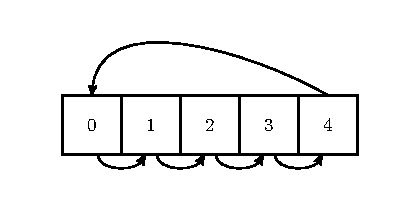
\includegraphics{00_7_imagem_2}
%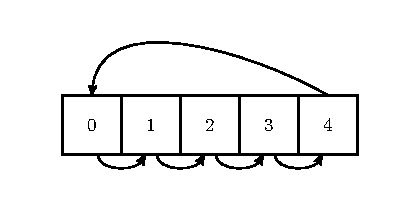
\includegraphics[scale=1.4]{00_7_imagem_2}
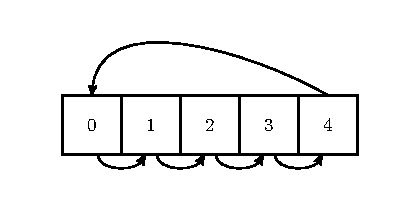
\includegraphics[width=.7\textwidth]{00_7_imagem_2}
\caption{Fluxograma do programa.}
\end{figure}

Na figura acima, podemos ver o quadrados representando um elemento da lista final (da lista embaralhada), onde os números representam os indices da lista e começamos pelo 0 por estarmos utilizando Python.
As setas mostram quem vai ter quem como amigo oculto, por exemplo, o nome que estiver no indice 1 terá a pessoa com nome no indice 2 como seu amigo oculto.




%\texttt{numpy}






